\section{Local System}
\label{sec:local-system-1}
In this section, the local system implementation is discussed, walking through
its most fundamental aspects.

\subsection{Buildroot configuration}
\label{sec:buildr-conf}
Buildroot is a tool to build custom tailored embedded Linux systems through
cross-compilation, easing the creation and deployment of such systems to be
loaded in the target system.
The base configuration resides in the Buildroot installation path. As a first
step the default configuration for a specific target must be generated running
\texttt{make <TARGET\_ARCH\_defconfig>}. Then, \texttt{make menuconfig} can be
executed to provide a \gls{gui} to interface the configurations of the custom
embedded Linux image.

The fundamental configurations for the project are:
\begin{item-c}
\item \emph{system configuration}: Enabling root login with password; Run a login
  prompt after boot;
\item \emph{filesystem images}: selection of file format and size for the image;
\item \emph{Toolchain}: setup of the development toolchain for the target,
  defining the C library and thread library debugging.
\item \emph{Network}: setup of the network utilities such as \texttt{dropbear}
  and \texttt{dhcpd} to ease the \gls{tcp-ip} communication with the target.
\item \emph{Packages}: setup of the relevant packages for the project, namely,
  \texttt{opencv4} for image acquisition and processing, \texttt{Qt} for
  \gls{ui}, \texttt{libcurl} to download ads, and \texttt{libcamera} to
  interface the \gls{csi} camera of the Raspberry Pi. 
\end{item-c}

After setting the \texttt{Buildroot} configurations, the target image is
generated using \texttt{make} and, if successful, it can be loaded into the
target platform.


Fig.~\ref{fig:build-cfg-4} through Fig.~\ref{fig:buildroot-cfg-4} presents the
Buildroot setup of some features using the \texttt{make menuconfig} utility.
% 
\begin{figure}[htb!]
\centering
    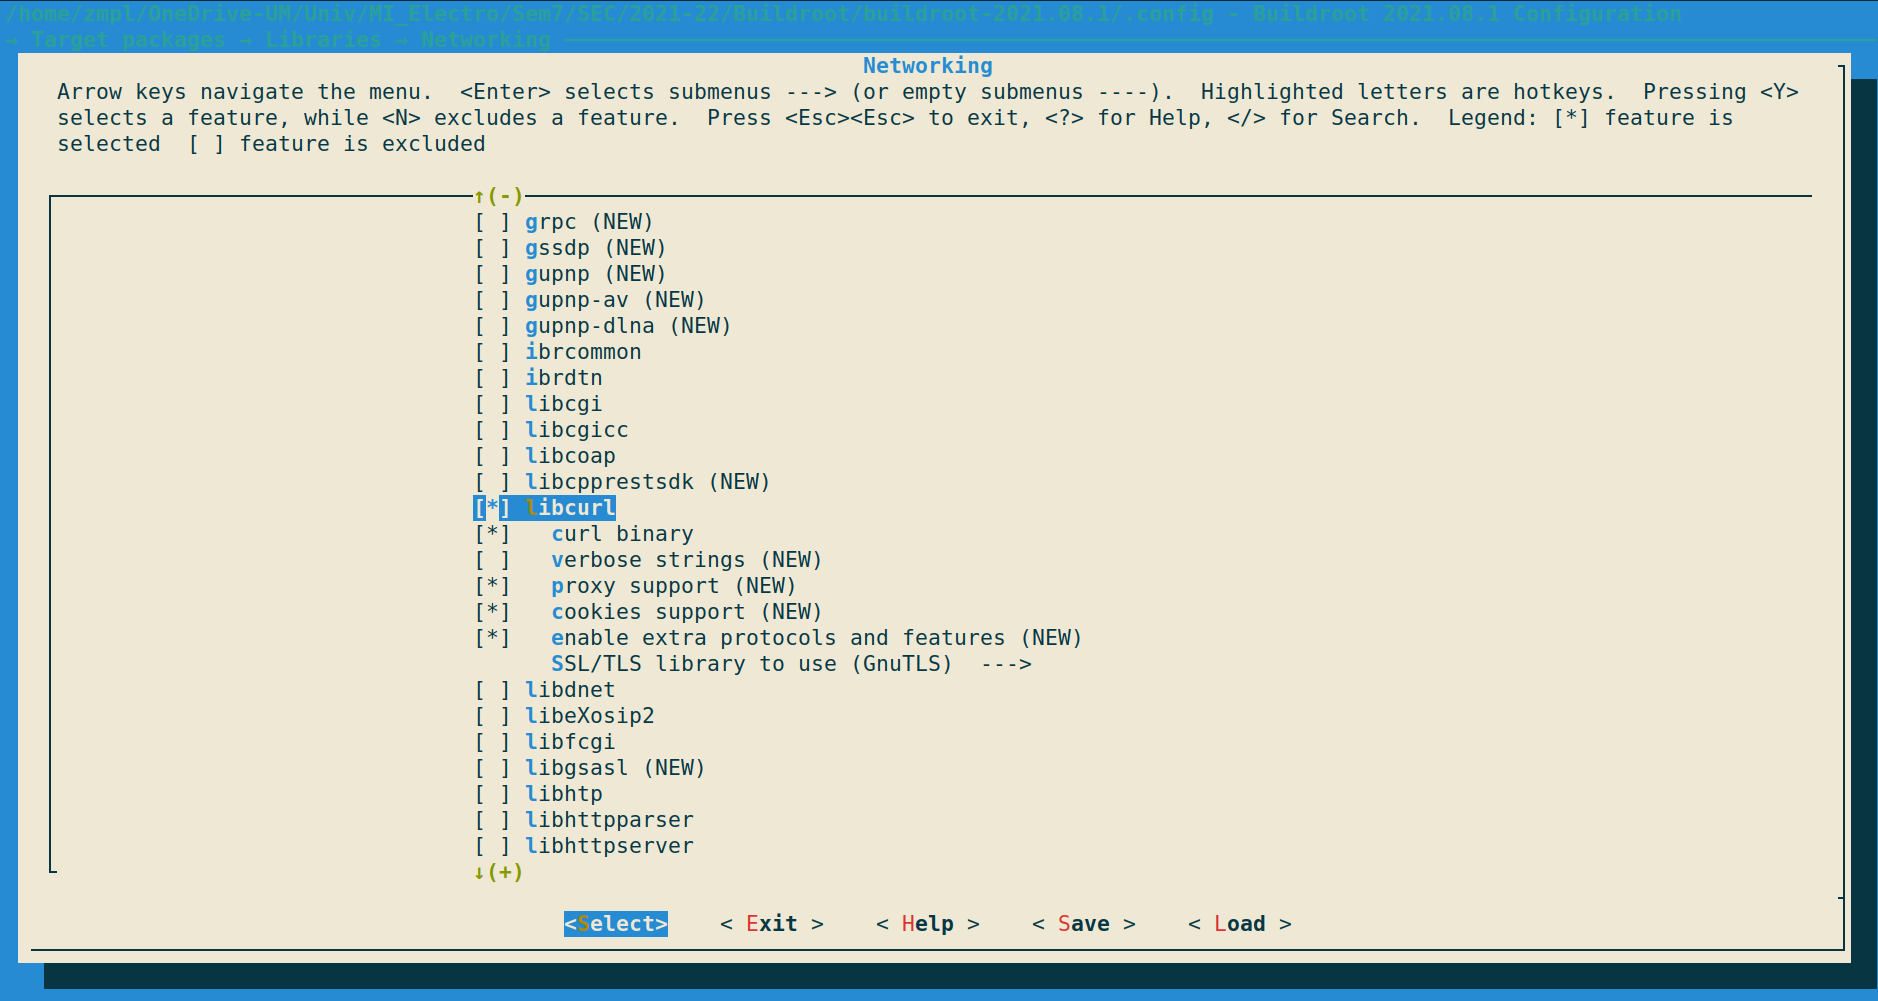
\includegraphics[width=0.8\columnwidth]{./img/buildroot-cfg-1.png}
  \caption{Buildroot setup: libcurl}%
\label{fig:buildroot-cfg-1}
\end{figure}
% 
\begin{figure}[htb!]
\centering
    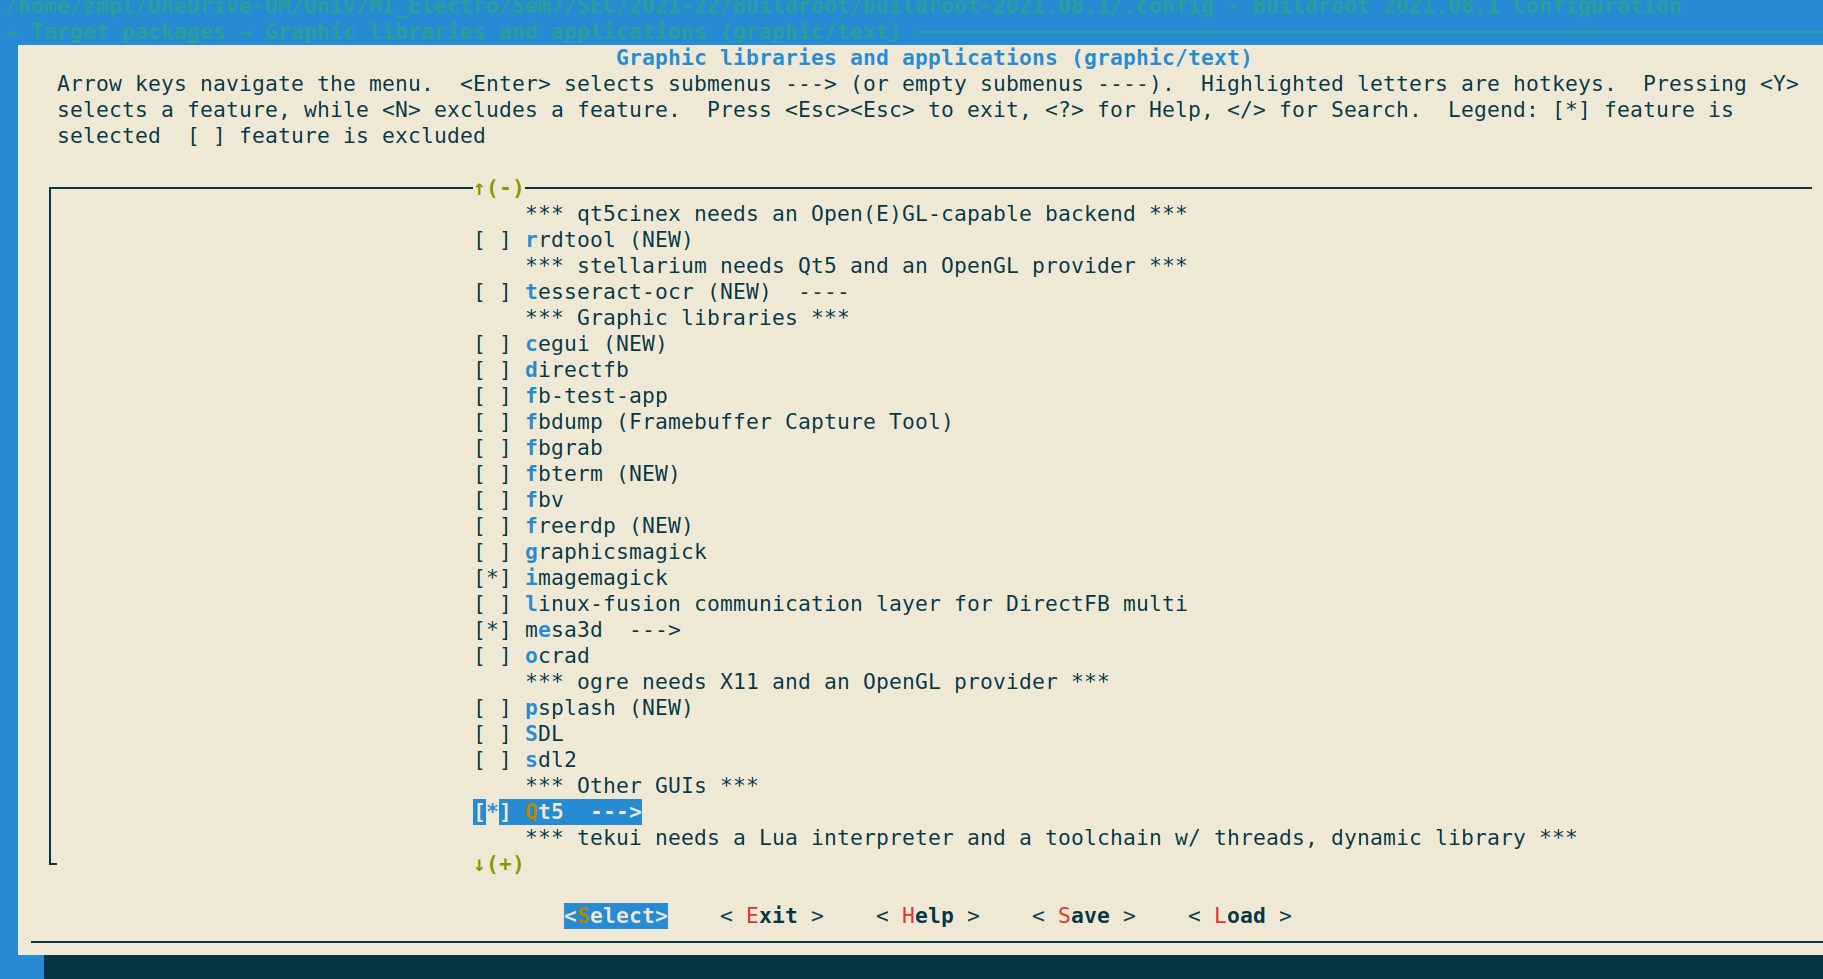
\includegraphics[width=0.8\columnwidth]{./img/buildroot-cfg-2.png}
  \caption{Buildroot setup: Qt5}%
\label{fig:buildroot-cfg-2}
\end{figure}
% 
\begin{figure}[htb!]
\centering
    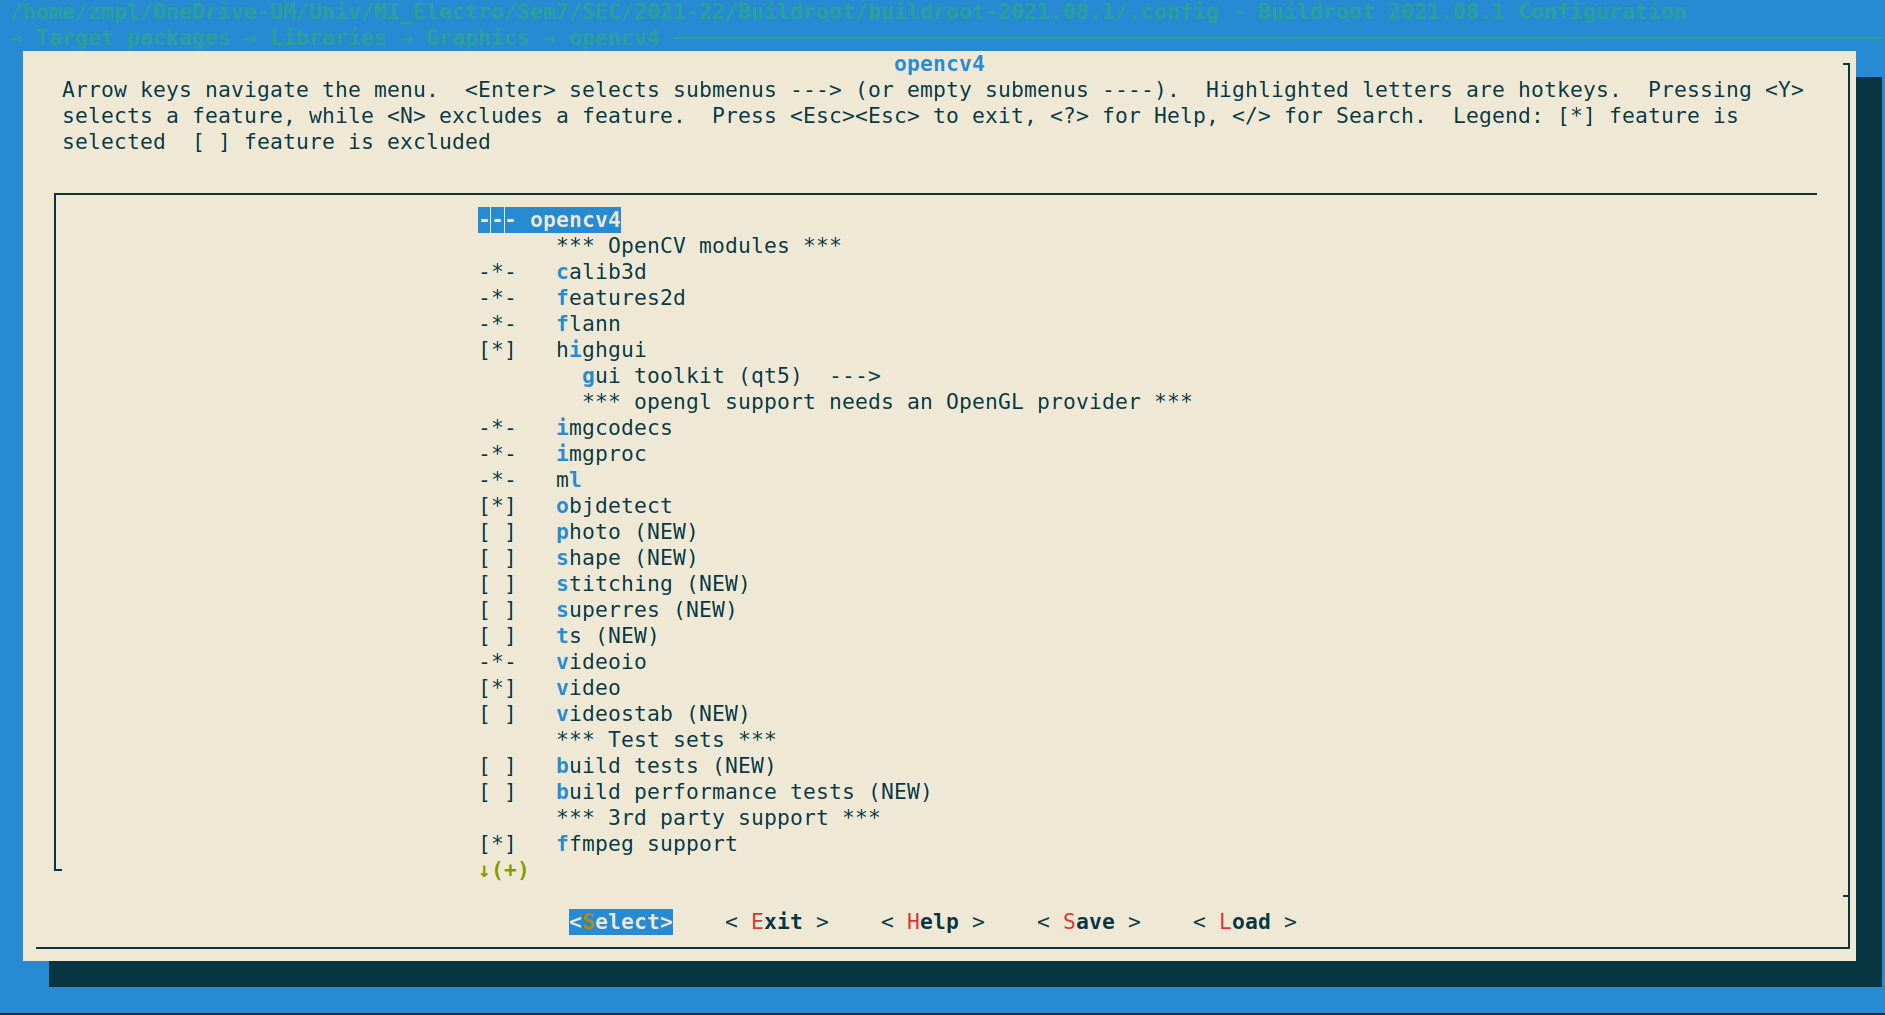
\includegraphics[width=0.8\columnwidth]{./img/buildroot-cfg-3.png}
  \caption{Buildroot setup: Opencv4}%
\label{fig:buildroot-cfg-3}
\end{figure}
% 
\begin{figure}[htb!]
\centering
    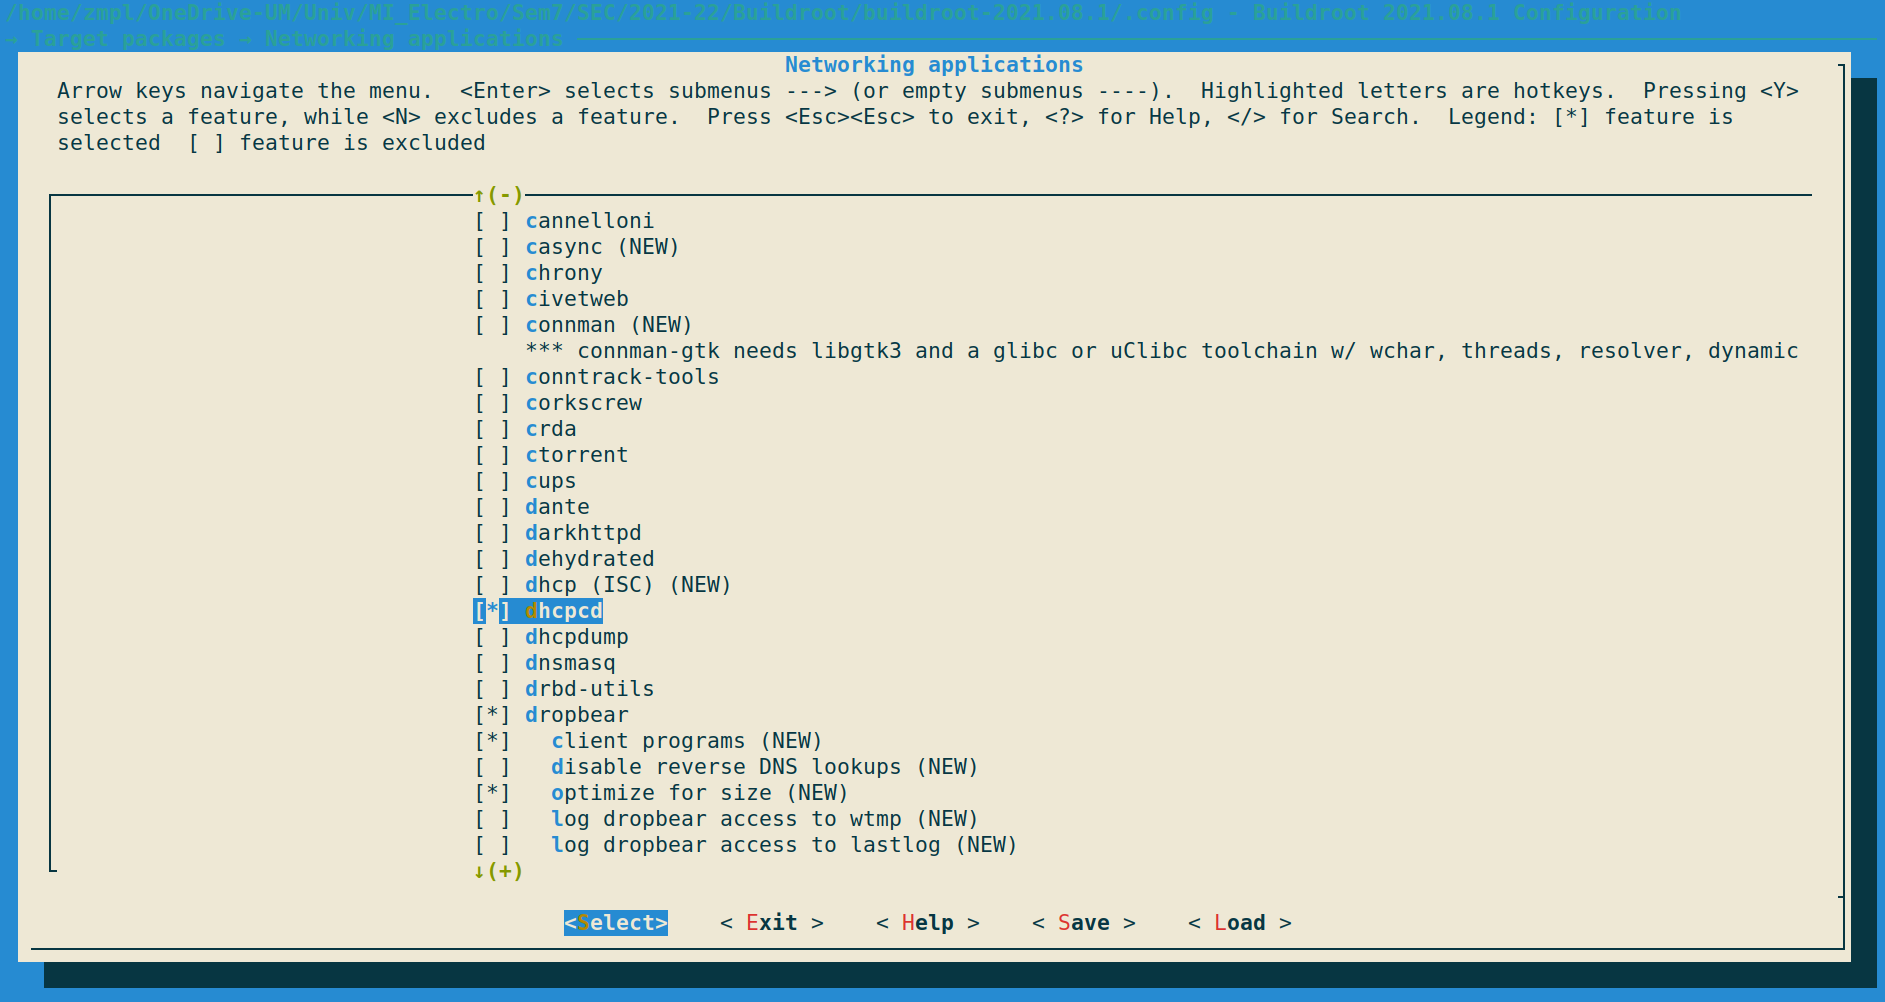
\includegraphics[width=0.8\columnwidth]{./img/buildroot-cfg-4.png}
  \caption{Buildroot setup: Networking}%
\label{fig:buildroot-cfg-4}
\end{figure}


\subsection{Automated build system for Local system software}
\label{sec:buildr-conf}
To build the \texttt{Local System} software an automated build tool was used,
namely \texttt{CMake}. \texttt{CMake} is a cross-platform tool to control the
software compilation process using platform and compiler independent
configuration files, and generating native \texttt{makefiles} to be executed,
building the required targets. For this purpose, a \texttt{CMakeLists.txt}
configuration file must be created in the software's path, as illutrated in Listing~\ref{lst:cmake-main}.

\lstinputlisting[language=c,
%firstline=1, lastline=3,
caption={\texttt{CMakeLists.txt} file: main build configuration file},
label=lst:cmake-main,
style=customc]{./listing/CMakeLists.txt}

Additionally, \texttt{CMake} provides better cross-compilation capabilities, by
enabling the programmer to specify the path to a toolchain configuration file,
keeping the original file general and delegating the specific compilation tools
for this file, as illustrated in Listing~\ref{lst:cmake-toolchain}.

\lstinputlisting[language=c,
%firstline=1, lastline=3,
caption={\texttt{raspToolchain.cmake} file: toolchain setup file},
label=lst:cmake-toolchain,
style=customc]{./listing/rasptoolchain.cmake}


%%% Local Variables:
%%% mode: latex
%%% TeX-master: "../../../dissertation"
%%% End:

\subsection{System initialization}
\label{sec:syst-init}
Embedded systems are typically self-contained and must be started without human
intervention, thus requiring an initialization scripted. The \texttt{inittab}
file contains the initialization scripts. In this file a line is added to
redirect to the initialization script of the \texttt{Local system}.
The process is relatively straightforward: adding modules to the \texttt{Linux}
kernel, setting up \gls{ipc} communication mechanisms like messages queues,
inserting the device driver modules into the \texttt{Linux} kernel, starting
daemons, running initialization commands (e.g., rotating the screen view), and
finally launching the main application.

\lstinputlisting[language=bash,
%firstline=1, lastline=3,
caption={Initialization script},
label=lst:init-sh,
style=make-pretty]{./listing/S_LS_Init.sh}

\subsection{Device drivers}
\label{sec:device-drivers-1}
Two device drivers were developed/adapted for fragrance diffusion and user
detection using two ultrasonic sensors. The device driver for user detection is
instantiated twice (in different \gls{hw} pins obviously), and then a daemon is
responsible to read periodically from these device drivers and assert if an user
was detected by counting these events in a sliding time window.

\subsubsection{Fragrance diffusion}
\label{sec:fragrance-diffusion}
The fragrance diffusion device driver must write to a specific pin to
enable/disable the device. The pin is statically defined in the module, thus
requiring recompilation for several diffuser actuators. In the future, this
should be changed to provide a more versatile interface. The module contains all
the typical functions associated with \texttt{static struct file\_operations},
namely \texttt{read}, \texttt{write}, \texttt{close} and \texttt{open}, although
the first is not required. The most important function is the \texttt{write}
one, which, upon writing to the associated file descriptor, sets the associated
pin state to \texttt{0} or \texttt{1}.
An excerpt of this device is illustrated
in Listing~\ref{lst:frag-module}.

\lstinputlisting[language=c,
%firstline=1, lastline=3,
caption={Fragrance diffuser kernel module (excerpt)},
label=lst:frag-module,
style=customc]{./listing/DDrivers/Frag/fragmodule.c}

\subsubsection{Ultrasonic sensor}
\label{sec:ultrasonic-sensor}
A device driver was implemented for the ultrasonic sensor, which can be
instantiated multiple times (in this case two), requiring the trigger and echo
pins, and the associated timeout. This device driver operates by emitting a
trigger signal and measuring the time between the trigger and echo signal to
determine the time of flight, and consequently the distance. Thus, this device
driver requires a specific signal timing as aforementioned in
Section~\ref{sec:motion-detection}..

The device driver implemented was adapted
from~\cite{hc-sro4-dd}, being ported to a more updated version, and abstracting
it. The most important functions are shown in
Listing~\ref{lst:uss-module}. Multiple device drivers can be instantiated or
removed in different hardware pins on demand, providing a more flexible
interface through the \texttt{sysfs\_configure\_store} function.
Then, on the background a periodic task performs the measurement ---
\texttt{do\_measurement} --- and when the echo is triggered a signal an
interruption is issued to handle this event, flushing the result to the
associated file descriptor.

It should be noted that for the present use case both triggers are shared,
as we expect to have `simultaneous' readings to work with.

\lstinputlisting[language=c,
%firstline=1, lastline=3,
caption={Ultrasonic sensor kernel module (excerpt) --- adapted from~\cite{hc-sro4-dd}},
label=lst:uss-module,
style=customc]{./listing/DDrivers/USS/hc-sro4.c}

\subsection{Daemons}
\label{sec:daemons-1}
As aforementioned, a daemon was created to periodically read the ultrasonic
sensors and count the detection events in a time sliding window, defining such
event as both sensors must be enabled. The daemon follows the required
initialization steps to detach itself from the outside world, as mentioned in
Section~\ref{sec:daemons}. Next, the message queue associated with the daemon is destroyed if present and
then (re)created.
Then, it should read the sensors periodically,
applying a sliding window and signaling the user detection event to a message
queue shared with the main application. The main application should periodically
consume this information to trigger the appropriate event handling. This daemon
is illustrated in Listing~\ref{lst:uss-daemon}.

\lstinputlisting[language=c,
%firstline=1, lastline=3,
caption={User detection daemon},
label=lst:uss-daemon,
style=customc]{./listing/Daemon/ussdaemon.cpp}

\subsection{Classes}
\label{sec:classes}
In these sections the main classes for the \texttt{Local System} are discussed.

\subsubsection{UI}
\label{sec:ui}
The \gls{ui} classes handle the interaction between the user and the application
and are defined according to the application mode, namely:
\begin{item-c}
\item \texttt{MainWindow}: main application's window. Manages all other windows
  (views), being the controller. The other views emit signals that are handled
  by these class to avoid circular dependencies and centralize the control.
\item \texttt{NormalWindow}: handles the Normal Window view application logic.
\item \texttt{InterWindow}: handles the Interaction Window view application logic.
\item \texttt{ImgFilterWindow}: handles the Image Filtering view application
  logic.
\item \texttt{SharWindow}: handles the Sharing view application logic.
\end{item-c}

In order to ease this model of control, the subordinate views are restricted to
a small subset of the application window, i.e., the only part that actually
requires replacing in each view. This means that the canvas to display the
images and the status bar is preserved throughout the application and solely
belongs to the \texttt{MainWindow}.

\paragraph{\textbf{NormalWindow}}
An example of a subordinate view is the \texttt{NormalWindow} which interface is
presented in Listing~\ref{lst:norm-wind}. It can be seen that it contains
a \texttt{Qt signal} to indicate when \texttt{Normal view} must be exited, and
it was used to test the application logic. This \texttt{Qt signal} is then
connected to the callback of a recipient object (a \texttt{slot}) to perform
some action.

\lstinputlisting[language=c,
%firstline=1, lastline=3,
caption={\texttt{NormalWindow} --- an example of a subordinate view},
label=lst:norm-wind,
style=customc]{./listing/LSApp/normalwindow.h}

\paragraph{\textbf{MainWindow}}
It is the view controller and the application logic manager, holding the
definition for each of the modes.
Listing~\ref{lst:main-wind} presents the interface for this class.

\lstinputlisting[language=c,
%firstline=1, lastline=3,
caption={\texttt{MainWindow} --- interface},
label=lst:main-wind,
style=customc]{./listing/LSApp/mainwindow.h}

It is
composed of several objects, namely:
\begin{item-c}
\item subordinate views (windows);
\item video capture
\item threads
\item mutexes: for synchronization
\item pEvents: wrapper around condition variables; for synchronization
\item image filters
\item scenes: welcome, video, and interaction
\item GIF
\item Twitter
\item Post: Twitter post
\item Video Player
\item Ad: current ad
\item Fragrance: current fragrance, fragrance manager to determine fragrance
  settings from the database, a diffuser and the associated timer for actuation
\item Timer: for periodic tasks
\item Socket: to connect to remote system
\item Message queue to interface the user detection sensors via daemon
\end{item-c}

It provides functions to:
\begin{itemize}
\item handle subordinate views signals and other relevant events like taking a
  picture, sharing a post, connection to the remote, receiving data from remote
  system, etc.
\item Handle computer vision tasks: grab frames, display images, detect faces,
  recognize gestures to navigate the interface and apply filters.
\item Thread workers: functions associated to each thread.
\item Twitter authentication
\item GIF creation
\item Handling communication
\item and several helpers
\end{itemize}

The threads and the associated workers will be detailed later.

\subsubsection{Ad}
\label{sec:ad}
This class handles ad logic, namely (see Listing~\ref{lst:ad}):
\begin{item-c}
\item storing relevant data
\item saving to and restoring data from the database
\item Retrieving important data like the filterID, the fragID, the timeslot, or
  the enabled state.
\item Enabling the Ad, dispatching it for execution in the normal mode,
  obviously if there is no user interaction.
\end{item-c}
It is important to note that this class is thread safe as it includes a
synchronization mechanism --- a mutex --- to prevent unattended access.

\lstinputlisting[language=c,
%firstline=1, lastline=3,
caption={\texttt{Ad} --- interface},
label=lst:ad,
style=customc]{./listing/LSApp/ad.h}

\subsubsection{DigitalOutput}
\label{sec:digitaloutput}
This class, enclosed in the \texttt{Device::Driver} namespace, models a digital
output device driver, as the fragrance diffuser. It provides methods to open,
write and close the device driver, as illustrated in Listing~\ref{lst:ddDigitalOut}.

\lstinputlisting[language=c,
%firstline=1, lastline=3,
caption={\texttt{DigitalOut} --- interface},
label=lst:ddDigitalOut,
style=customc]{./listing/LSApp/ddDigitalOut.h}

\subsubsection{Fragrance classes}
\label{sec:fragrance-classes}
The fragrance classes, enclosed in the \texttt{Fragrance} namespace, handle the
fragrance logic, namely, creating, diffusing and managing it.

\paragraph{\textbf{Frag}}
The \texttt{Frag} class defines a Fragrance as illustrated in
Listing~\ref{lst:frag}. It allows to calculate the durations of the enabled and
disabled state of the fragrance diffuser associated with it, and besides the
normal getters and setters, it provides methods to serialize and deserialize
this object, enabling it to be saved and loaded from the database.

\lstinputlisting[language=c,
%firstline=1, lastline=3,
caption={\texttt{Frag} --- interface},
label=lst:frag,
style=customc]{./listing/LSApp/frag.h}

\paragraph{\textbf{fragDiffuser}}
The fragrance diffuser class associates a fragrance with the respective device
driver, enabling it to appropriately handle the requirements of each
fragrance (see Listing~\ref{lst:fragDiffuser}).
It is important to note that this class is thread safe as it includes a
synchronization mechanism --- a mutex --- to prevent unattended access.

\lstinputlisting[language=c,
%firstline=1, lastline=3,
caption={\texttt{fragDiffuser} --- interface},
label=lst:fragDiffuser,
style=customc]{./listing/LSApp/fragDiffuser.h}

\paragraph{\textbf{fragManager}}
The \texttt{FragManager} classes manages the fragrance database containing its
settings (see Listing~\ref{lst:fragManager}).
It is important to note that this class is thread safe as it includes a
synchronization mechanism --- a mutex --- to prevent unattended access.

\lstinputlisting[language=c,
%firstline=1, lastline=3,
caption={\texttt{fragManager} --- interface},
label=lst:fragManager,
style=customc]{./listing/LSApp/fragManager.h}

\subsubsection{ImgFilter}
\label{sec:imgfilter}
The \texttt{ImgFilter} class wraps the image filter functionality, mainly as a
container
(see Listing~\ref{lst:imgFilter}).

\lstinputlisting[language=c,
%firstline=1, lastline=3,
caption={\texttt{imgFilter} --- interface},
label=lst:imgFilter,
style=customc]{./listing/LSApp/imgfilter.h}

\subsubsection{msgQueue}
\label{sec:msgqueue}
The \texttt{msgQueue} class provides an abstraction over the Linux system calls
to ease the usage of this \gls{ipc} mechanism
(see Listing~\ref{lst:mqueue}).

\lstinputlisting[language=c,
%firstline=1, lastline=3,
caption={\texttt{msgQueue} --- interface},
label=lst:mqueue,
style=customc]{./listing/LSApp/msgqueue.h}

\subsubsection{pEvent}
\label{sec:msgqueue}
The \texttt{pEvent} class provides an abstraction over the pthread condition
variables, comprising the loosely named POSIX Event. This class enables to emit
and receive signals in a much more straightforward way, but always ensuring its
integrity, as it is protected by a mutex
(see Listing~\ref{lst:pEvent}).

\lstinputlisting[language=c,
%firstline=1, lastline=3,
caption={\texttt{pEvent} --- interface},
label=lst:pEvent,
style=customc]{./listing/LSApp/pEvent.h}

\subsubsection{Post}
\label{sec:post}
The \texttt{Post} class handles the Twitter posts, containing the message and
the associated media type
(see Listing~\ref{lst:post}).

\lstinputlisting[language=c,
%firstline=1, lastline=3,
caption={\texttt{Post} --- interface},
label=lst:post,
style=customc]{./listing/LSApp/post.h}

\subsection{Threads}
\label{sec:threads}
This section addresses the Local System threads, illustrated in Listing~\ref{lst:threads}.

\lstinputlisting[language=c,
%firstline=1, lastline=3,
caption={Local system threads},
label=lst:threads,
style=customc]{./listing/LSApp/threads.cpp}

\subsubsection{frameGrab}
\label{sec:framegrab}
The \texttt{frameGrab} thread is responsible for acquiring a camera frame and
feeding the computer vision engine to detect faces, recognize gestures, or apply
image filters. It checks the mode and if adequate the frame is captured and
dispatched for further processing.

\subsubsection{Rx and ProcessRx}
\label{sec:rx}
The \texttt{Rx} and \texttt{ProcessRx} threads work together following the
producer--consumer model: the first receives data frames from the Remote System
and pushes it to a shared buffer, signaling this event to the \texttt{ProcessRx}
thread;
the second consumes these data frames, parsing them, and signaling the relevant
events, like downloading an Ad.

\subsubsection{gifSave}
\label{sec:gifsave}
The \texttt{gifSave} thread takes care of saving a GIF into disk. A thread is
required because this I/O operation can take a significant amount of time.

\subsubsection{DownloadAd}
\label{sec:downloadad}
The \texttt{downloadAd} thread takes care of downloading an ad and the
associated media through the proxy server \texttt{transfer.sh}. When the event
\texttt{ev\_download} is signaled, the current ad is retrieved and the ad is downloaded.

\subsubsection{Main thread}
\label{sec:main-thread}
The main thread belongs to the \texttt{UI}, and it responsible for processing
its events. Associated with this thread, a periodic task is executed to verify
the application mode and stimulate the application (see
Listing~\ref{lst:periodicTask}), namely: checking normal mode, checking if a
user was detected, or if a remote connection was lost.

\lstinputlisting[language=c,
%firstline=1, lastline=3,
caption={Main thread periodic task: checkMode},
label=lst:periodicTask,
style=customc]{./listing/LSApp/periodicTask.cpp}
